% talk with nice pictures /mnt/backup/safe-with-time/torben/safed/0321/talk/talk.lisp  amazingly i wrote this presentation in lisp!
% theory /mnt/backup/safe-with-time/torben/safed/0417
% WP6 D6.6 Report on DIC experiments /mnt/backup/safe-with-time/torben/safed/1125
\chapter{DIC}
\lstdefinelanguage{Maxima}{
keywords={addrow,addcol,zeromatrix,ident,augcoefmatrix,ratsubst,diff,ev,tex,%
with_stdout,nouns,express,depends,load,submatrix,div,grad,curl,%
rootscontract,solve,part,assume,sqrt,integrate,abs,inf,exp},
sensitive=true,
comment=[n][\itshape]{/*}{*/}
}
\lstset{language=Maxima}

\citep{Schwertner2008}

\begin{figure}[htbp]
  \centering
  \includegraphics[width=4cm]{dic-refocused-maximum-angle}
  \caption{}
  \label{fig:dic-refocused-maximum}
\end{figure}


\begin{figure}[htbp]
  \centering
  \includegraphics[width=4cm]{dic-setup}
  \caption{}
  \label{fig:dic-setup}
\end{figure}


\begin{figure}[htbp]
  \centering
  \includegraphics[width=4cm]{dic_prism-white-bg}
  \caption{}
  \label{fig:dic_prism-white}
\end{figure}


\begin{figure}[htbp]
  \centering
  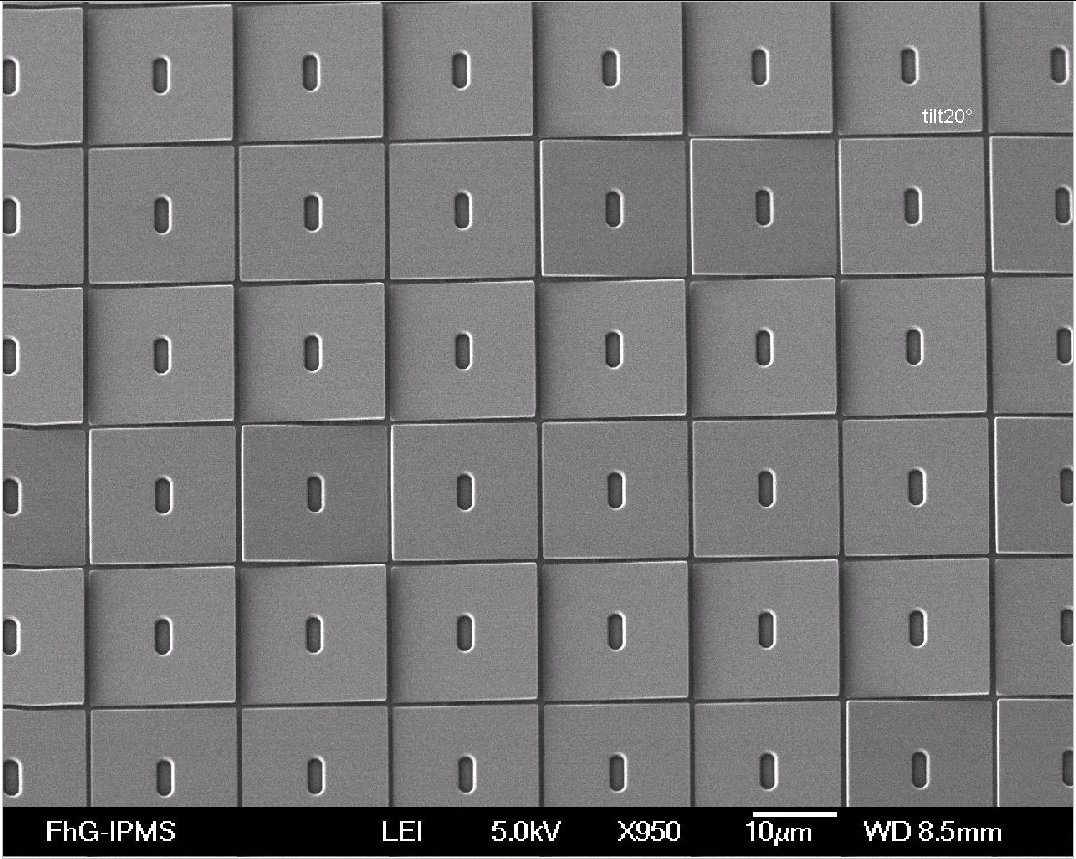
\includegraphics[width=4cm]{mma-tilts}
  \includegraphics[width=4cm]{mma_dic-shear}
  \caption{}
  \label{fig:mma-tilts}
\end{figure}

\begin{figure}[htbp]
  \centering
  \includegraphics[height=4cm]{dic-setup-sketch}
  \caption{}
  \label{fig:dic-setup-sketch}
\end{figure}

\begin{figure}[htbp]
  \centering
  \includegraphics[width=4cm]{mma-dic-unadjusted}
  \caption{}
  \label{fig:mma-dic-unadjusted}
\end{figure}
\begin{figure}[htbp]
  \centering
  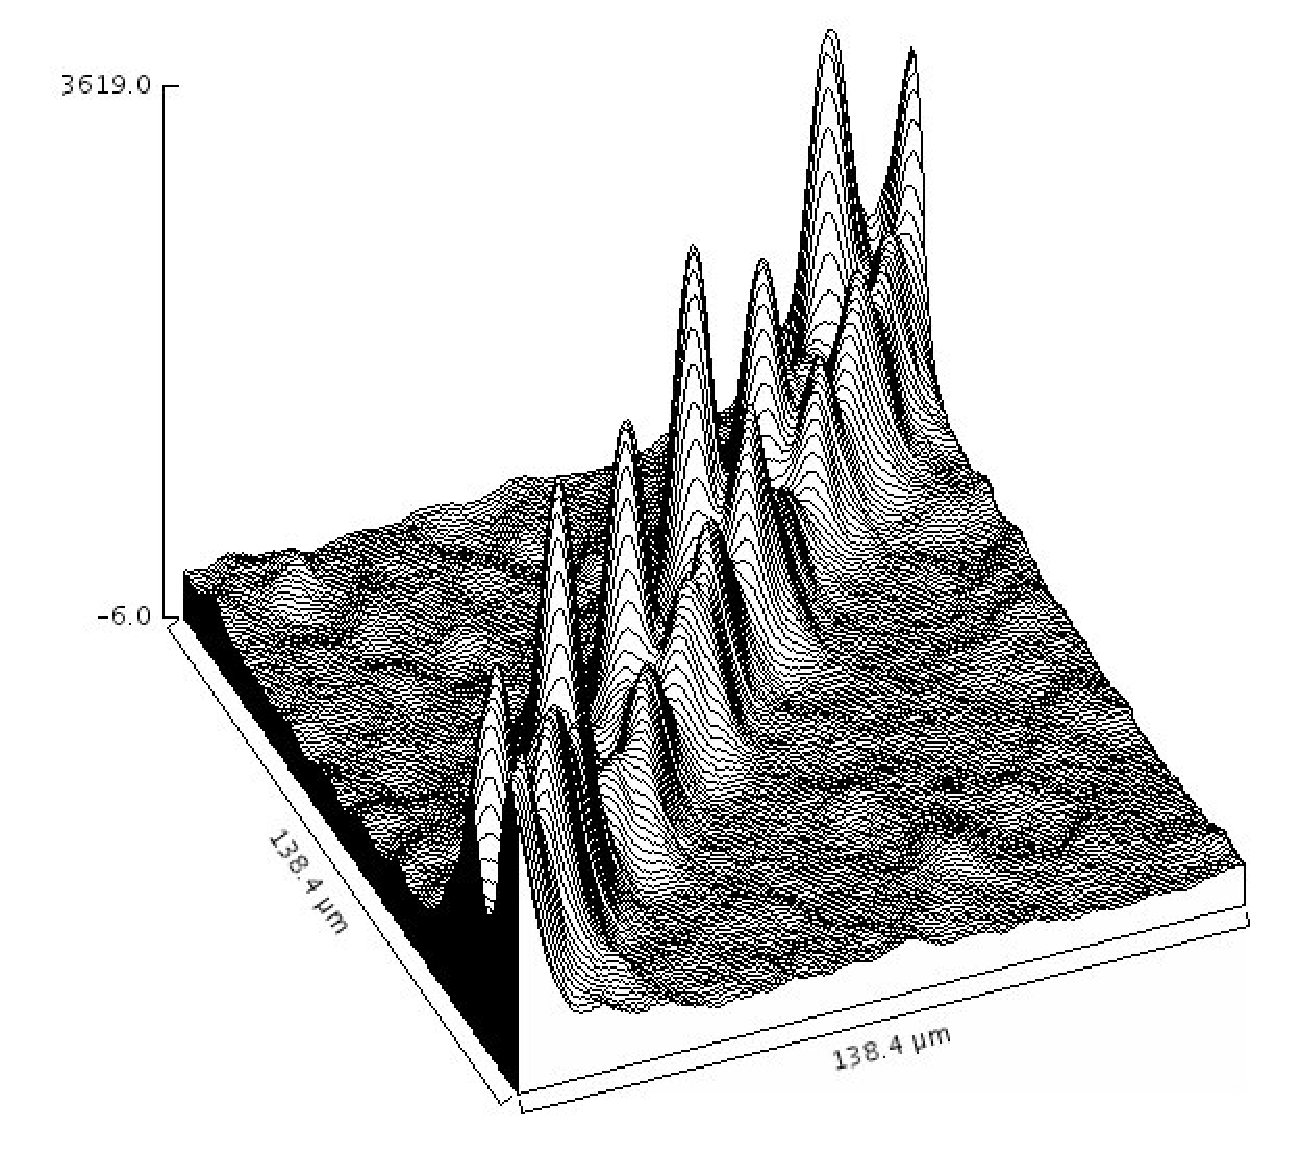
\includegraphics[width=4cm]{1checker-height}
  \caption{}
  \label{fig:1checker-height}
\end{figure}
\begin{figure}[htbp]
  \centering
  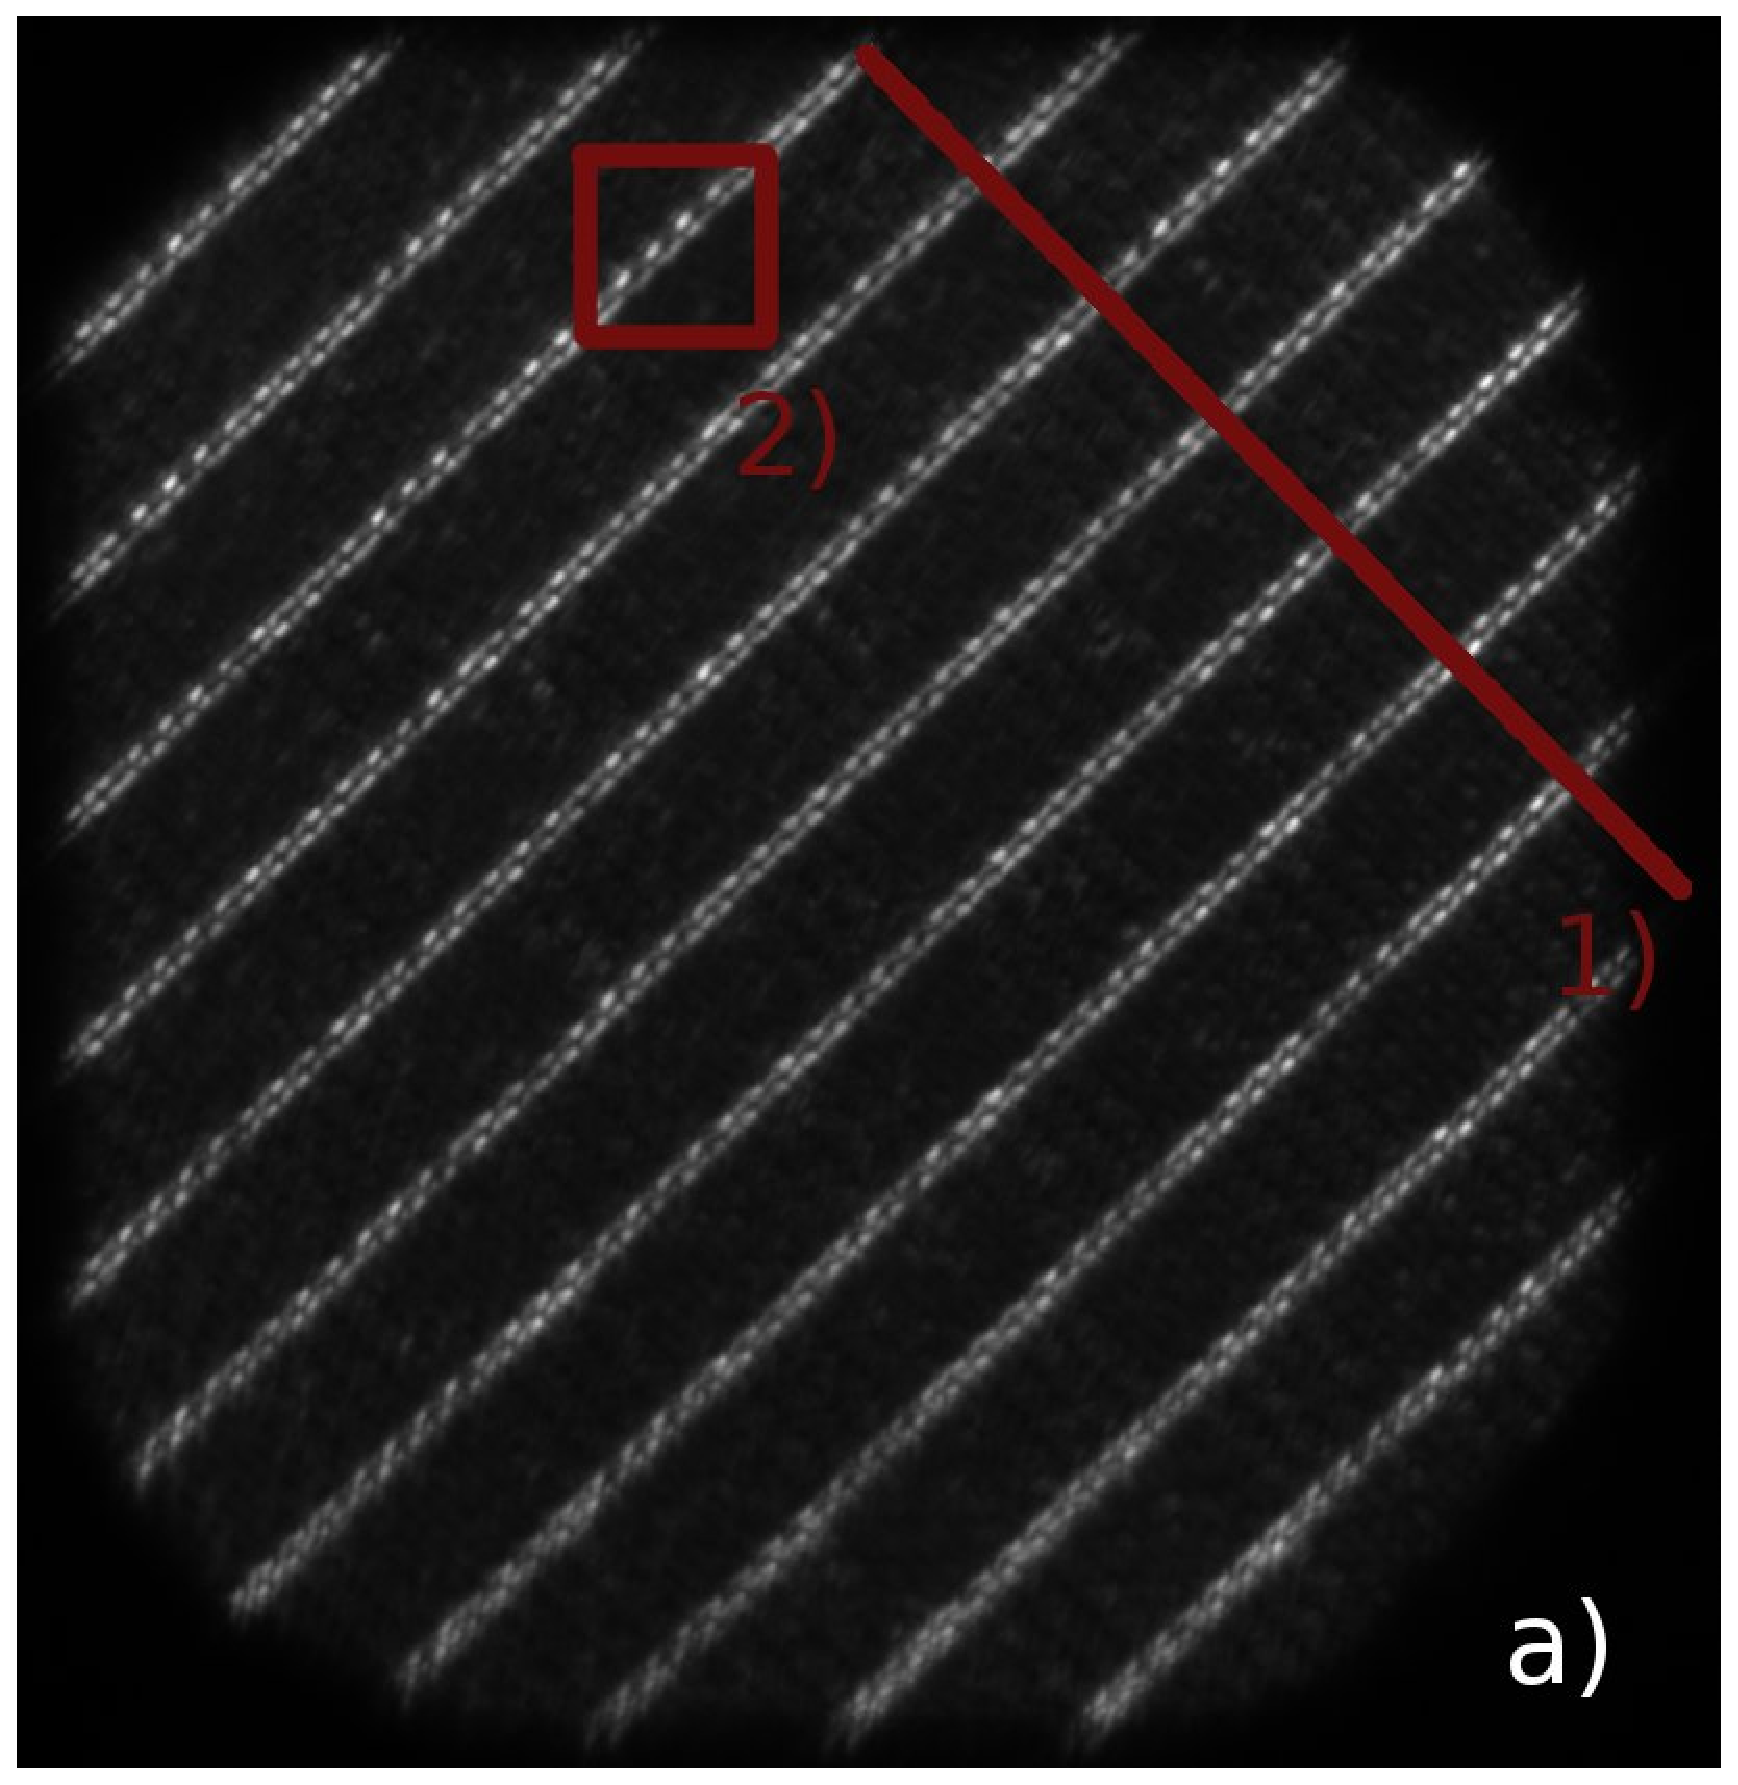
\includegraphics[width=4cm]{1checker}
  \caption{}
  \label{fig:1checker}
\end{figure}
\begin{figure}[htbp]
  \centering
  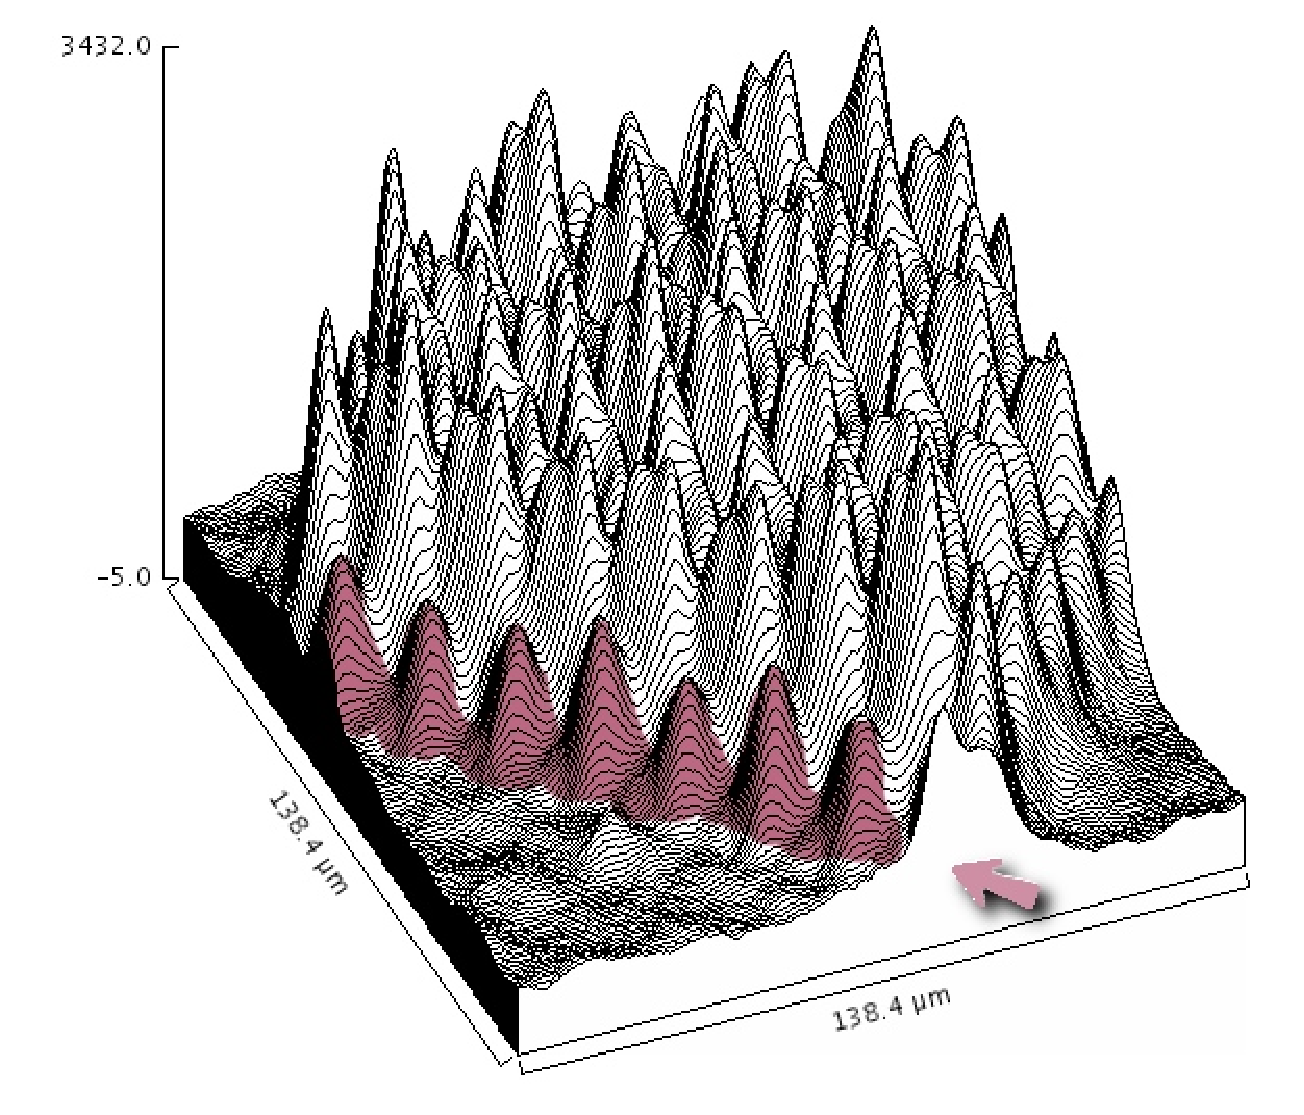
\includegraphics[width=4cm]{2checker-height-arrow}
  \caption{}
  \label{fig:height-arrow}
\end{figure}
\begin{figure}[htbp]
  \centering
  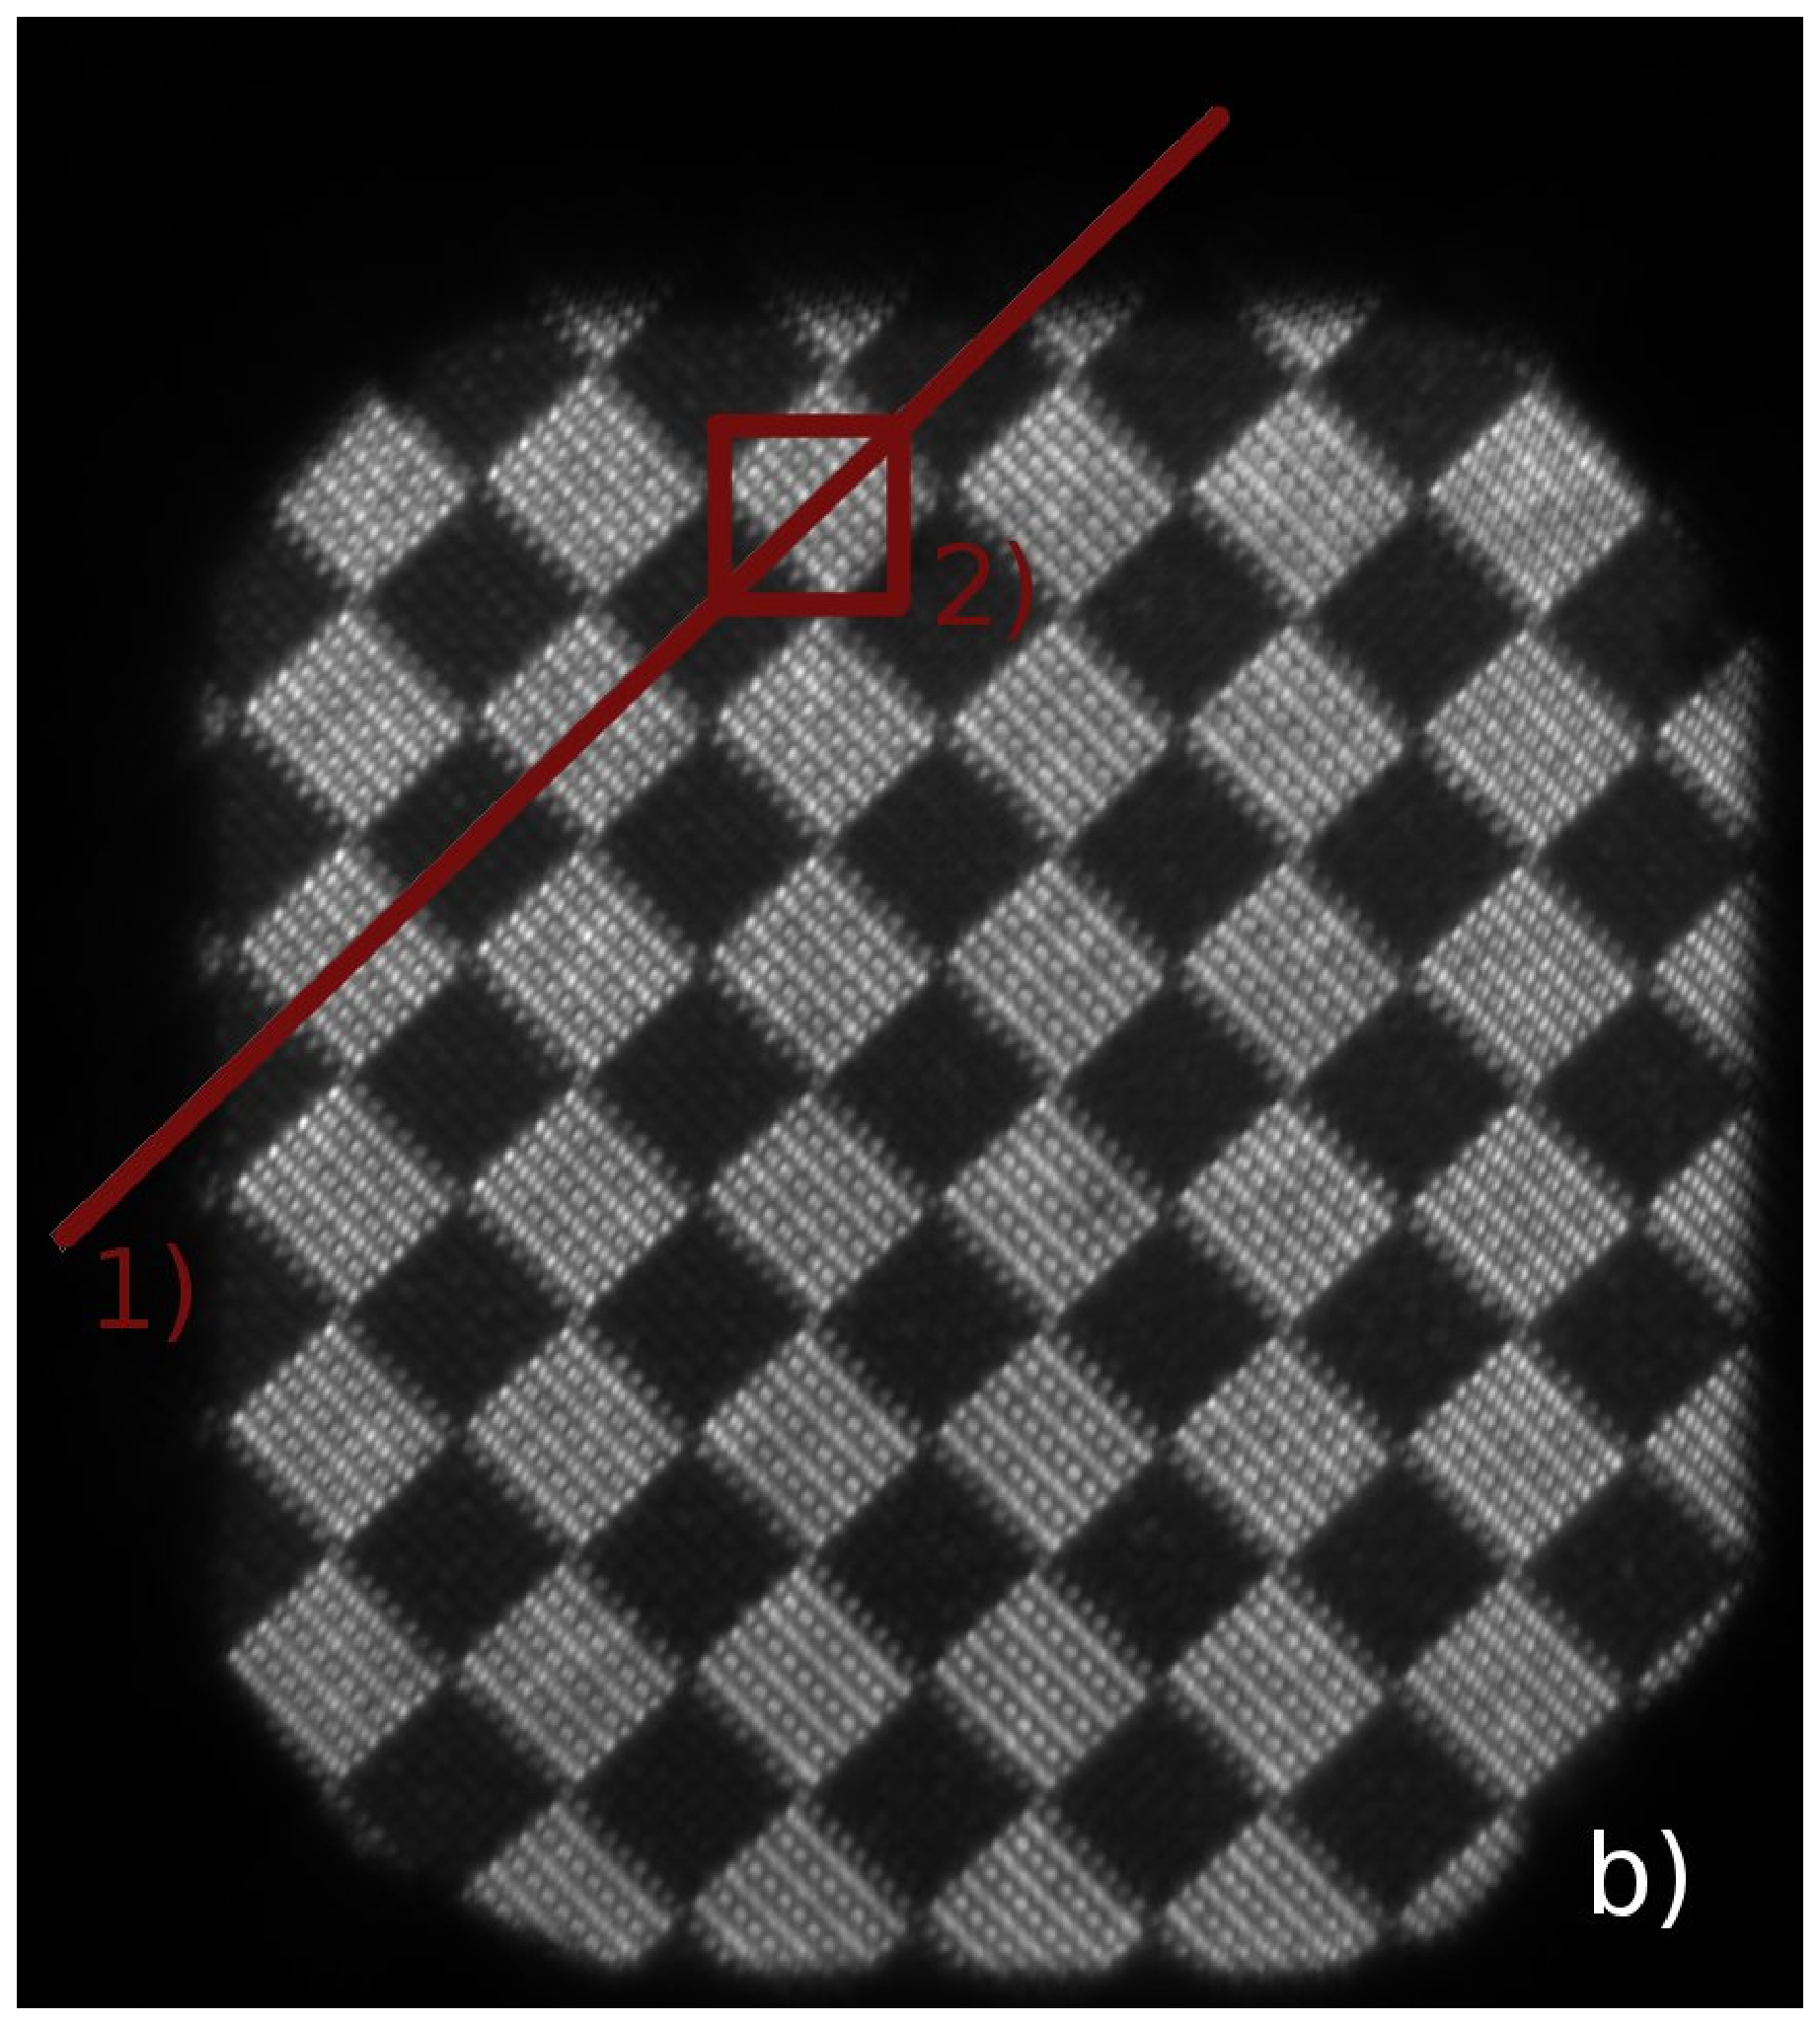
\includegraphics[width=4cm]{2checker}
  \caption{}
  \label{fig:2checker}
\end{figure}
\begin{figure}[htbp]
  \centering
  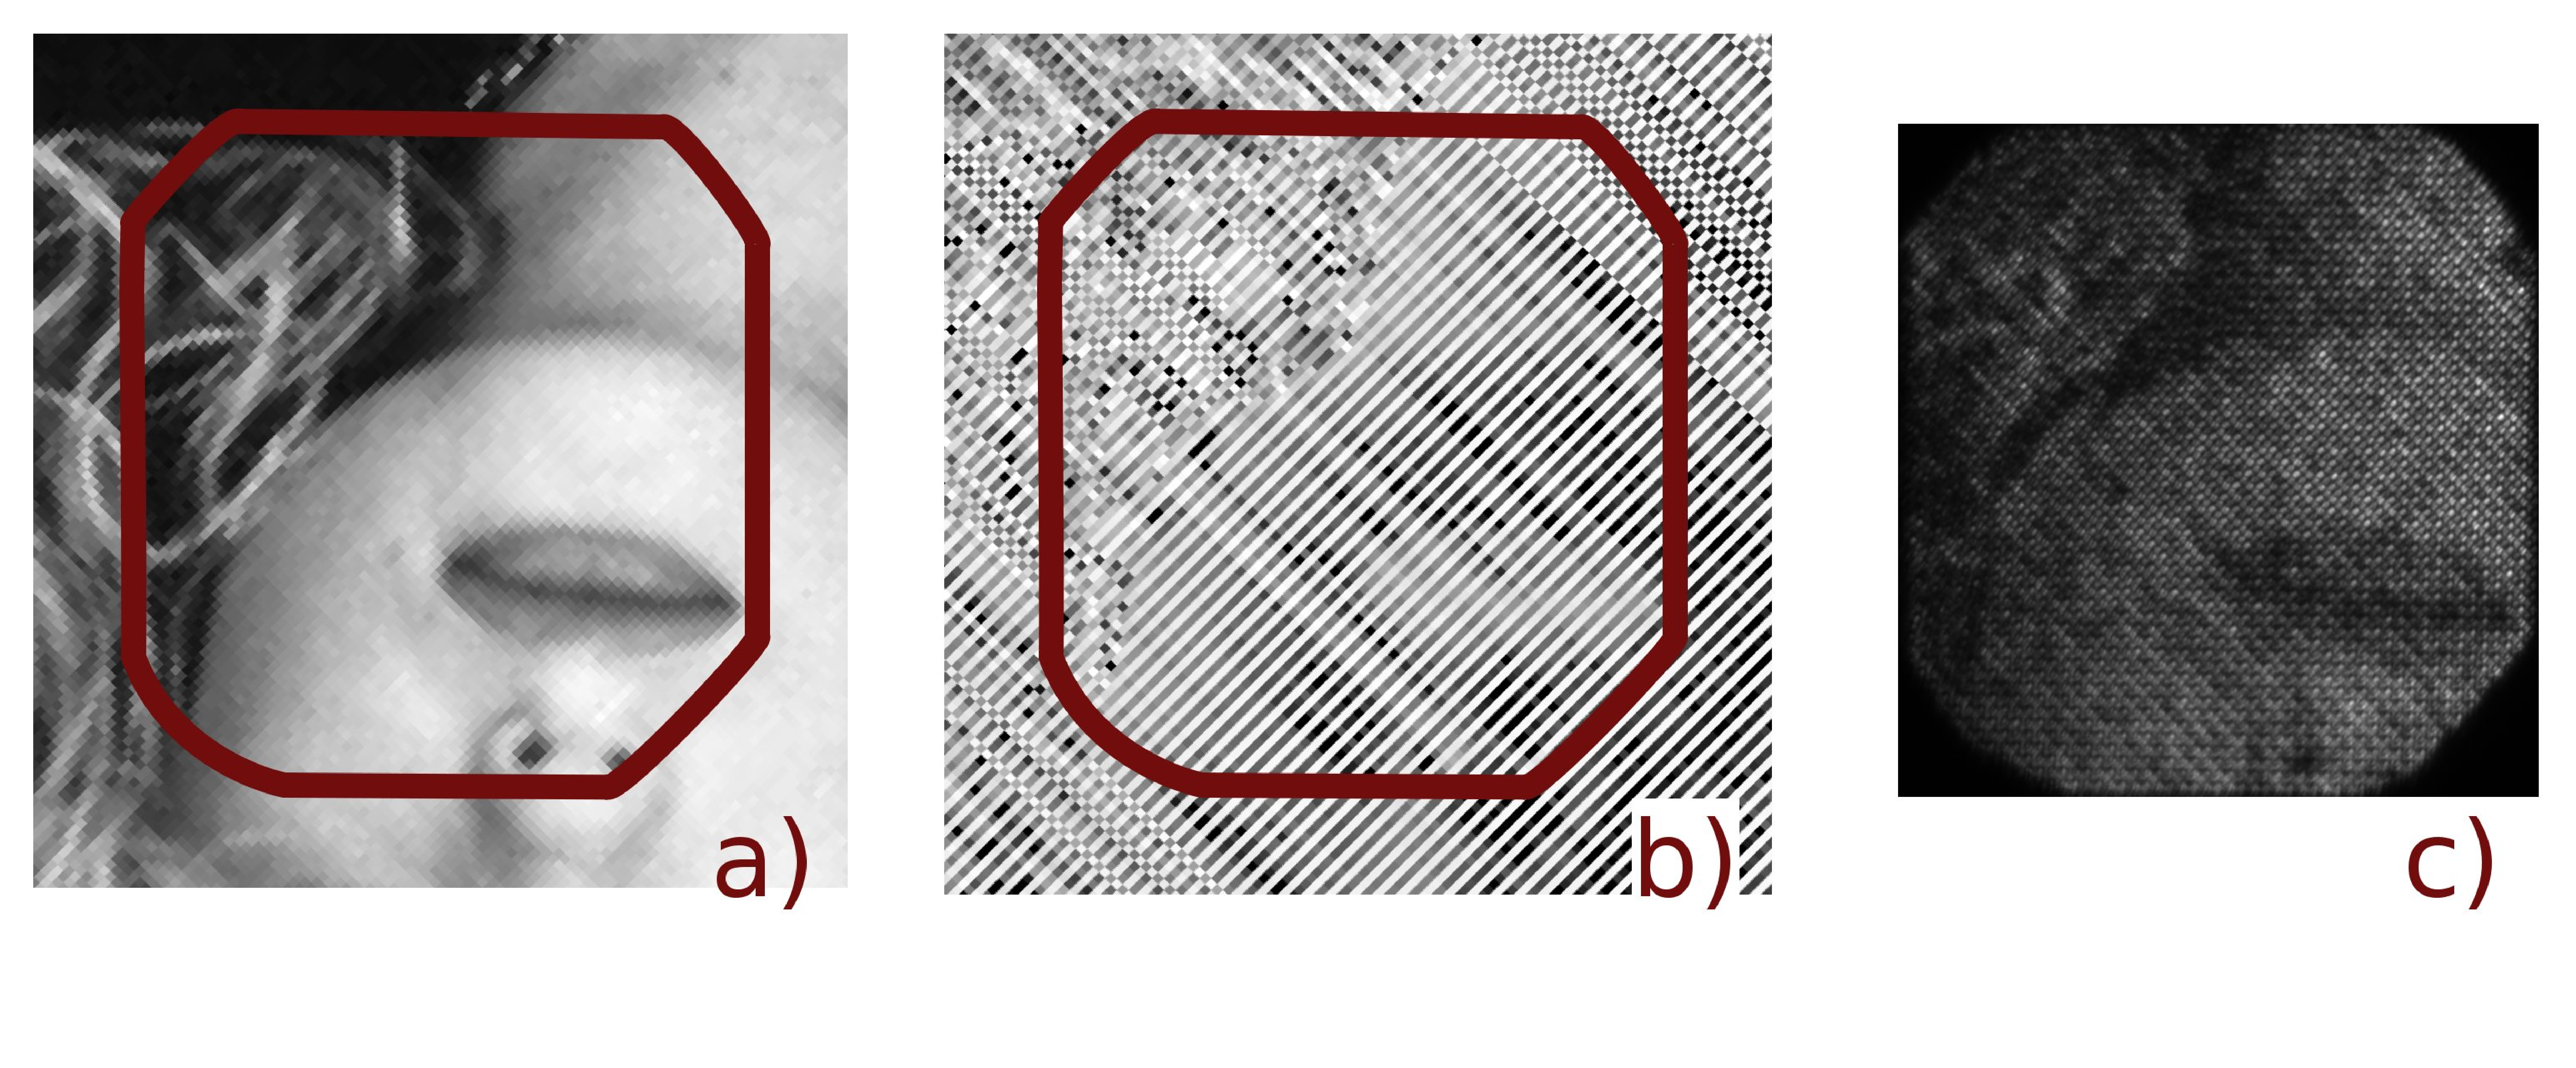
\includegraphics[width=4cm]{erika-detail}
  \caption{}
  \label{fig:detail}
\end{figure}

\begin{figure}[htbp]
  \centering
  \includegraphics[width=4cm]{erika-detail2}
  \caption{}
  \label{fig:detail2}
\end{figure}

\begin{figure}[htbp]
  \centering
  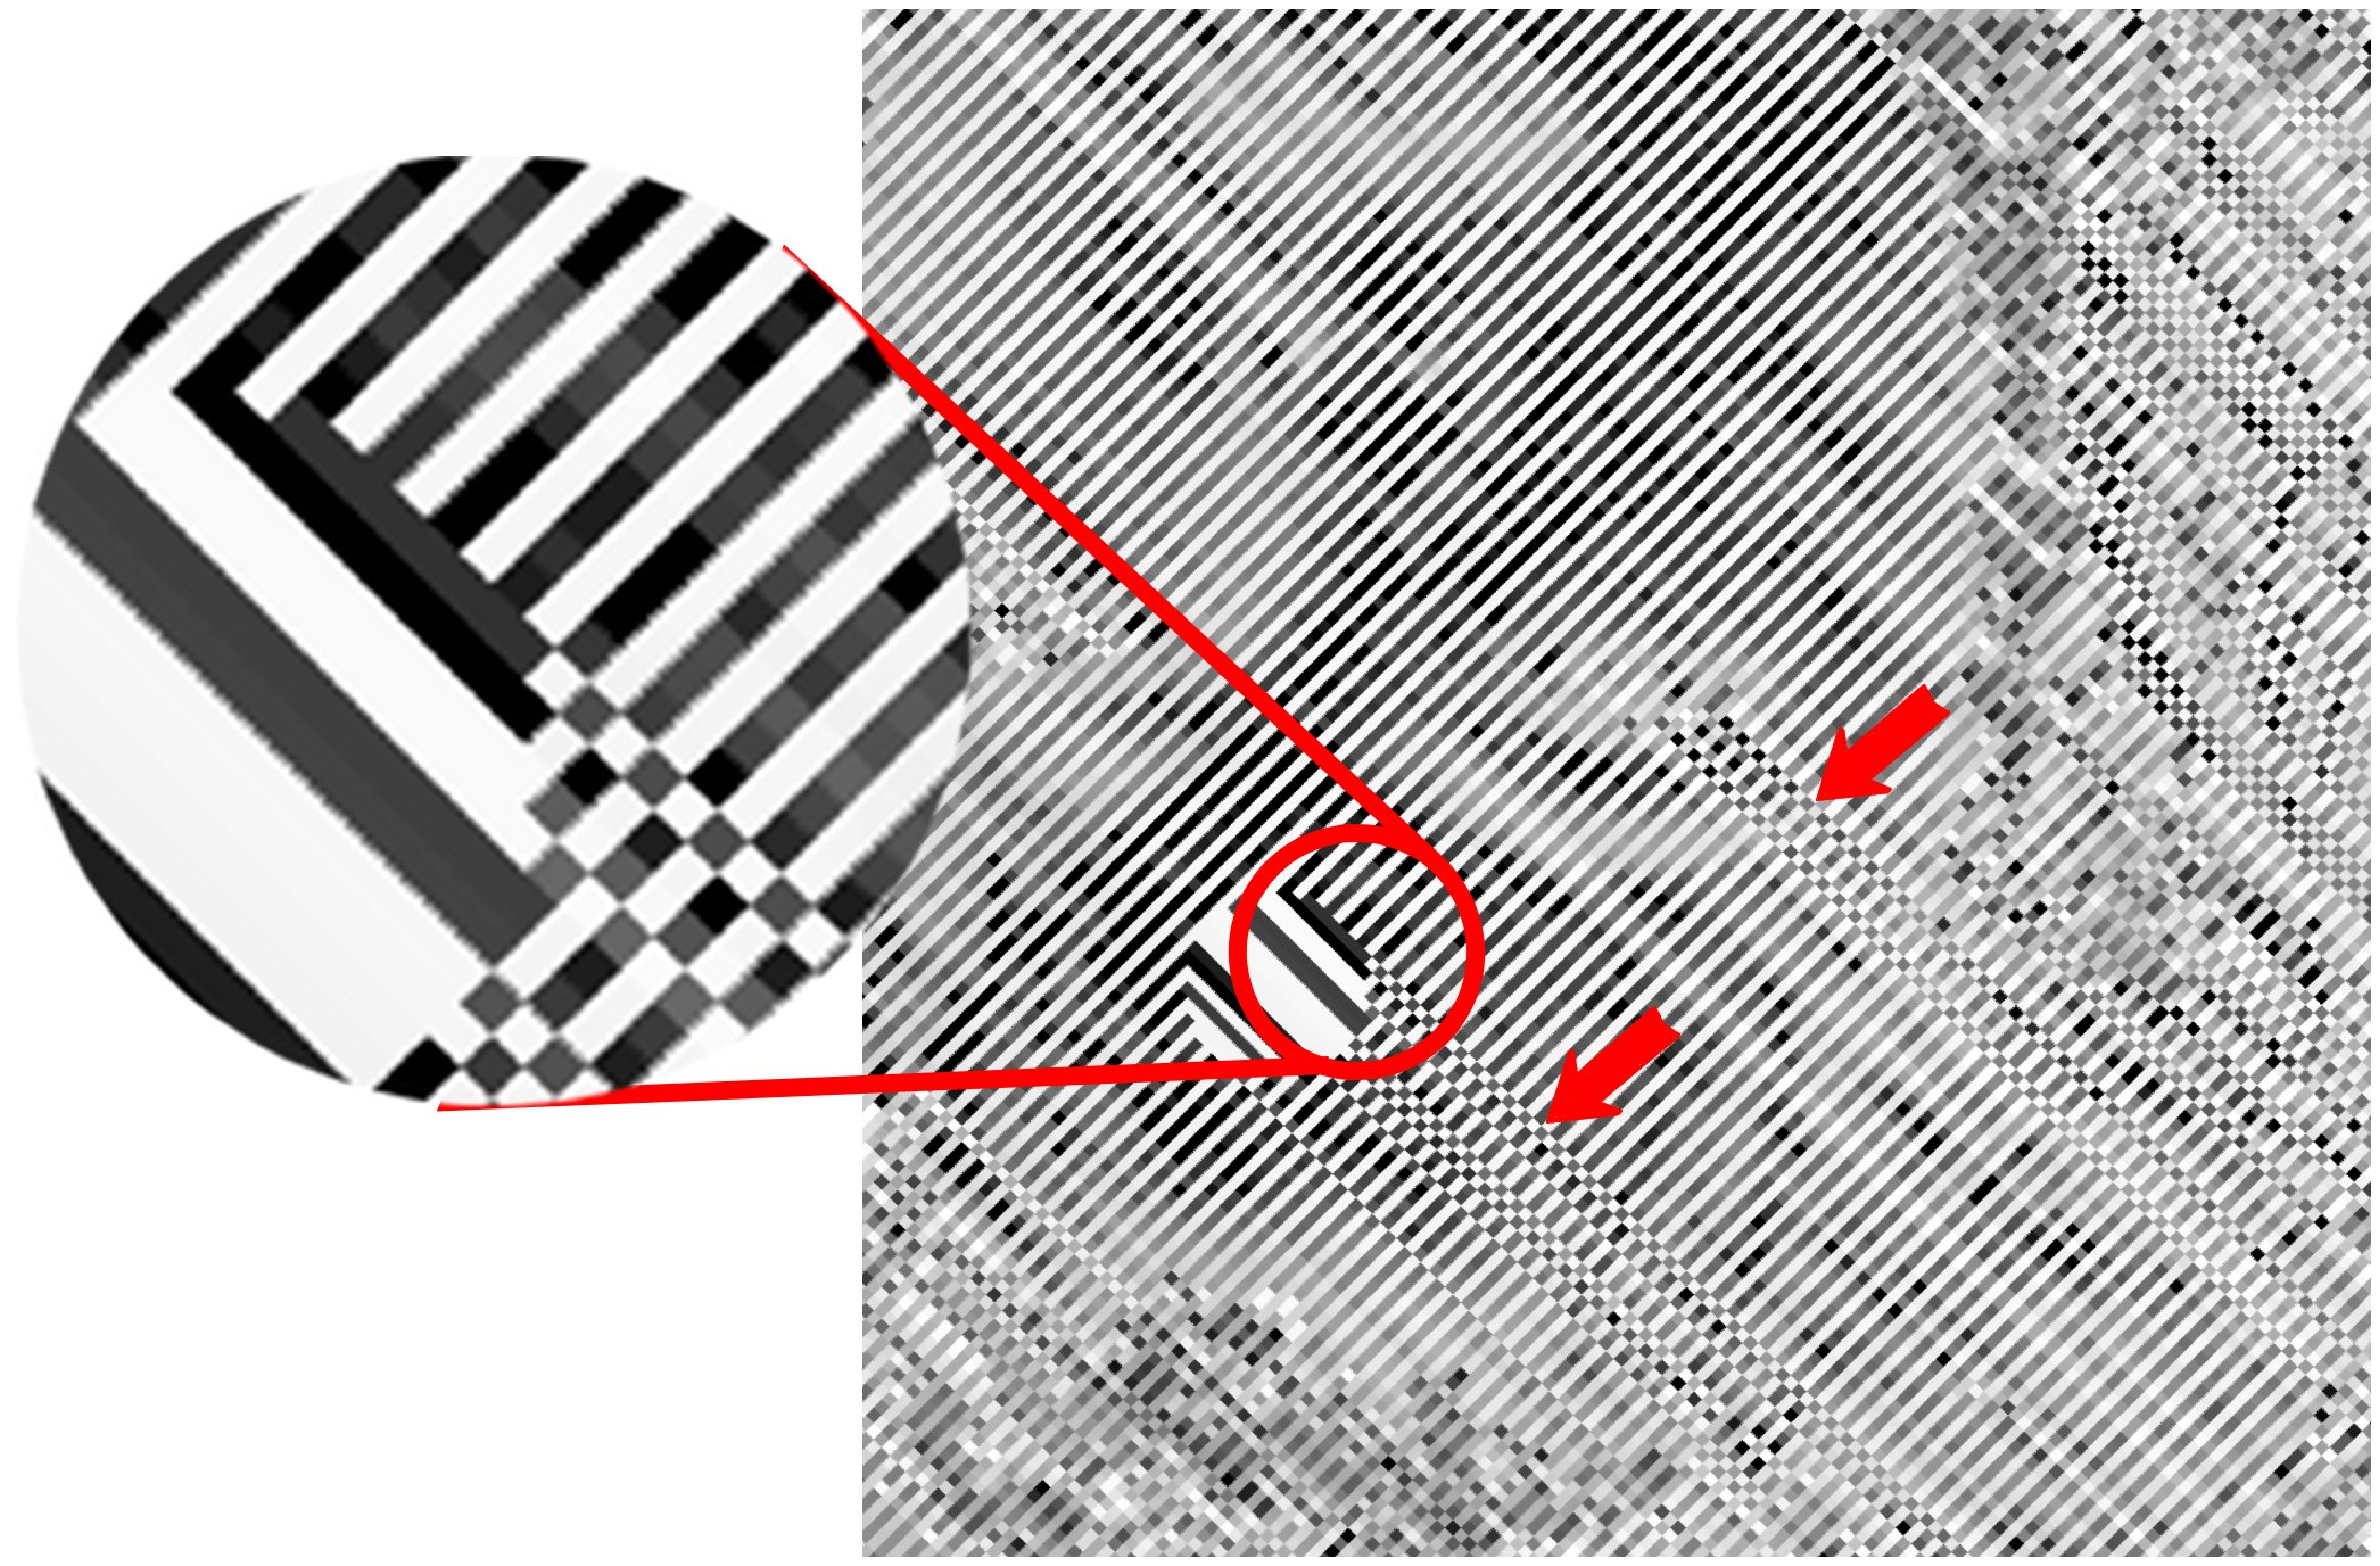
\includegraphics[width=4cm]{erika-streak-overview}
  \caption{}
  \label{fig:streak}
\end{figure}

\section{Abstract}
I describe the implementation of a simple raytracing algorithm for
uniaxial material.  The goal is to model a Wollaston prism and
estimate if it will be possible to use it for contrast enhancement of
a torsional micro-mirror array and to investigate what contrast we can
expect from the device.
\section{Description}
I want to design a Wollaston quartz prism that creates a split of
\unit[32]{mrad} between the two escaping beams.  A Wollaston prism is
a crystal plate consisting of two quartz wedges with an internal angle
$\alpha$. The right part of Figure 3 in \citep{Nomarski1960} shows the kind
of setup we intend to build. 
\begin{figure}[htbp]
  \centering
  \input{wollaston.eps_tex}
  \caption{Sketch of the raytrace through a Wollaston prism.}
\end{figure}
I take the names of the prisms from the Nomarski patent. I start the
trace with a beam that hits Q2 from the left. The optic axis of Q2 is
$\vect c_2=(0,1,0)^T$. It is perpendicular to the beam propagation. As
the ray enters the prism perpendicular to the front surface the
propagation angle doesn't change. However the ordinary beam is faster
than the extraordinary beam.

I calculate the refractive indizes of quartz with the formula given in
\citep{Ghosh1999}. For a wavelength of \unit[768]{nm} the refractive indices
are: $n_e=1.547916$ and $n_o=1.538998$.

At the contact surface between wedge Q1 and Q2 the ray direction for
ordinary and extraordinary beams change. Quartz is uniaxial
birefringent and optically active. Optical activity doesn't concern us
here it only has an important influence if the ray direction is in a
low angle to the optic axis (which will never occur in this Wollaston).

The calculation of the refracted wavevector and ray direction is
described in \citep{Lekner1991,Weidlich2008}. Here I implemented these
formulas in Maxima. I chose Maxima because I hope it will be easier to
switch to multiple precision which is necessary to calculate the phase
difference between rays. Apparrently not even 128-bit long-double
would be good enough for these calculations \cite{Lekner1991}. Knowing
the phase difference between the two beams is important to understand
if the prism will actually recombine zeroth and first order of the
micro-mirrors into a proper DIC image. I fear that the first order ray
might have a completely wrong phase leading to image artifacts and
very low contrast.

These two papers don't describe refraction at a
birefringent-birefringent interface. However I am not interested in
the exact Fresnel coefficients. I just start with one perfectly
polarized ray in Q1 and use the wavevector (the length $|\vect k_e|$
for $n_e(\theta)$) to calculate the direction in Q2 and the refractive
index there. I do this calculation twice. Once for the ray which is
polarized in the xz-plane and another time for the ray in the
yz-plane.  For the quartz-air interface I use the function raytrace2.
Its a copy of the birefringent solver but uses $n_e=n_o=1$. That's
easier than implementing a simple refraction formula for now.

The comments of the Maxima listing contain the results for an internal
wedge angle of 0.83 degrees. This angle was originally given to me by
the Comar polarization expert as an estimated angle needed to achieve
\unit[32]{mrad} between the exiting beams. Note that if my
calculations are correct it seems like he mixed up mrad and degree as
the angle between the two exiting beams is \unit[0.031]{degrees}.

\begin{lstlisting}
/*
uniaxial raytracer p0416/1991lekner_uniaxial.pdf
good repetition in p0415/2008weidlich_render-calcit.pdf
dispersion data for quartz  p0415/1999ghosh_quartz-calcite-dispersion-data.pdf
wollaston prism configuration for nomarski contrast (patent) Desktop2/NOMARSKI.pdf
*/

/* raytracer code according to 1991 lekner */

/* use a high precision */
showtime:false;
fpprec:800;
fpprintprec:25;
type:bfloat;

/* dispersion data from 1999 ghosh */
n_quartz_o2(l):=block(
  [a:1.28604141,
  b:1.07044083,
  c:1.00585997e-2,
  d:1.10202242,
  f:100,l2:l^2],
  a+b*l2/(l2-c)+d*l2/(l2-f));

n_quartz_e2(l):=block(
  [a:1.28851804,
  b:1.09509924,
  c:1.02101864e-2,
  d:1.15662475,
  f:100,l2:l^2],
  a+b*l2/(l2-c)+d*l2/(l2-f));

/* xi and phi give the direction of the optic axis
   theta is the angle of the incoming wavevector towards the surface normal
   n1 is the refractive index of medium for the incoming beam */
raytrace(lambda0,xi,phi,theta,n1):=block(
  [eo,ee,de,c,alp,bet,gam,k,kin,K,weg,q,q1,
  qo,No,Eo,so,d,qe,Ne,Ee,se,Eox,Eoy,Eoz,Eex,Eey,Eez,
  A,B,D,
  rss,rsp,tso,tse,
  qt,
  rpp,rps,tpo,tpe,
  ko,ke],
  eo:n_quartz_o2(lambda0),
  ee:n_quartz_e2(lambda0),
  de:ee-eo,
  /* orientation of optic axis */
  xi:xi*%pi/180,
  phi:phi*%pi/180,
  c:[sin(xi)*cos(phi),sin(xi)*sin(phi),cos(xi)],bfloat,
  c:c/sqrt(c.c),
  [alp,bet,gam]:c,
  /* incoming wavevector */
  n1:1,
  theta:theta*%pi/180,bfloat,
  k:2*%pi/lambda0,bfloat,
  kin:n1*k*[sin(theta),0,cos(theta)],
  [K,weg,q]:kin,
  q1:q,
  /* ordinary ray */
  qo:sqrt(eo*k^2-K^2),
  No:1/sqrt(bet^2*eo*k^2+(alp*qo-gam*K)^2),
  Eo:No*[-bet*qo,alp*qo-gam*K,bet*K],
  ko:[K,0,qo],
  so:ko/sqrt(ko.ko),
  /* ray direction se of extraordinary ray */
  d:eo*(ee*(eo+gam^2*de)*k^2-(ee-bet^2*de)*K^2),numer,
  qe:(sqrt(d)-alp*gam*K*de)/(eo+gam^2*de),
  Ne:No/k*1/sqrt(eo),
  Ee:Ne*[alp*qo^2-gam*qe*K,
         bet*eo*k^2,
         gam*(eo*k^2-qe^2)-alp*qe*K],
  ke:[K,0,qe],       
  se:[(alp*qe-gam*K)*(alp*qe*K-gam*(eo*k^2-qe^2))+bet^2*K*eo,
      bet*(alp*K+gam*qe)*(qe^2-qo^2),
      (alp*qe-gam*K)*(alp*qo^2-gam*qe*K)+bet^2*qe*eo*k^2],numer,
  se:se/sqrt(se.se),
  /* reflection and transmission coefficients for
  s-polarization at isotropic-birefringent interface */
  [Eox,Eoy,Eoz]:Eo,
  [Eex,Eey,Eez]:Ee,
  A:(qo+q1+K*tan(theta))*Eox-K*Eoz,
  B:(qe+q1+K*tan(theta))*Eex-K*Eez,
  D:(q1+qe)*A*Eey-(q1+qo)*B*Eoy,
  rss:((q1-qe)*A*Eoy-(q1-qo)*B*Eoy)/D,
  rsp:2*n1*k*(A*Eex-B*Eox)/D,
  tso:-2*q1*B/D,
  tse:-2*q1*A/D,
  /* coefficients for p-polarization */
  qt:q1+K*tan(theta),
  rpp:(2*qt/D)*((q1+qe)*Eox*Eey-(q1+qo)*Eex*Eoy),
  rps:2*n1*k*(qe-qo)*Eoy*Eey/D,
  tpo:2*n1*k*(q1+qe)*Eey/D,
  tpe:-2*n1*k*(q1+qo)*Eoy/D,
  [so,se,ko,ke]);

raytrace2(lambda0,xi,phi,theta,n1,n2):=block(
  [eo,ee,de,c,alp,bet,gam,k,kin,K,weg,q,q1,
  qo,No,Eo,so,d,qe,Ne,Ee,se,Eox,Eoy,Eoz,Eex,Eey,Eez,
  A,B,D,
  rss,rsp,tso,tse,
  qt,
  rpp,rps,tpo,tpe,
  ko,ke],
  eo:n2^2,
  ee:n2^2,
  de:0,
  /* orientation of optic axis */
  xi:xi*%pi/180,
  phi:phi*%pi/180,
  c:[sin(xi)*cos(phi),sin(xi)*sin(phi),cos(xi)],bfloat,
  c:c/sqrt(c.c),
  [alp,bet,gam]:c,
  /* incoming wavevector */
  n1:1,
  theta:theta*%pi/180,bfloat,
  k:2*%pi/lambda0,bfloat,
  kin:n1*k*[sin(theta),0,cos(theta)],
  [K,weg,q]:kin,
  q1:q,
  /* ordinary ray */
  qo:sqrt(eo*k^2-K^2),
  No:1/sqrt(bet^2*eo*k^2+(alp*qo-gam*K)^2),
  Eo:No*[-bet*qo,alp*qo-gam*K,bet*K],
  ko:[K,0,qo],
  so:ko/sqrt(ko.ko),
  /* ray direction se of extraordinary ray */
  d:eo*(ee*(eo+gam^2*de)*k^2-(ee-bet^2*de)*K^2),numer,
  qe:(sqrt(d)-alp*gam*K*de)/(eo+gam^2*de),
  Ne:No/k*1/sqrt(eo),
  Ee:Ne*[alp*qo^2-gam*qe*K,
         bet*eo*k^2,
         gam*(eo*k^2-qe^2)-alp*qe*K],
  ke:[K,0,qe],       
  se:[(alp*qe-gam*K)*(alp*qe*K-gam*(eo*k^2-qe^2))+bet^2*K*eo,
      bet*(alp*K+gam*qe)*(qe^2-qo^2),
      (alp*qe-gam*K)*(alp*qo^2-gam*qe*K)+bet^2*qe*eo*k^2],numer,
  se:se/sqrt(se.se),
  /* reflection and transmission coefficients for
  s-polarization at isotropic-birefringent interface */
  [Eox,Eoy,Eoz]:Eo,
  [Eex,Eey,Eez]:Ee,
  A:(qo+q1+K*tan(theta))*Eox-K*Eoz,
  B:(qe+q1+K*tan(theta))*Eex-K*Eez,
  D:(q1+qe)*A*Eey-(q1+qo)*B*Eoy,
  rss:((q1-qe)*A*Eoy-(q1-qo)*B*Eoy)/D,
  rsp:2*n1*k*(A*Eex-B*Eox)/D,
  tso:-2*q1*B/D,
  tse:-2*q1*A/D,
  /* coefficients for p-polarization */
  qt:q1+K*tan(theta),
  rpp:(2*qt/D)*((q1+qe)*Eox*Eey-(q1+qo)*Eex*Eoy),
  rps:2*n1*k*(qe-qo)*Eoy*Eey/D,
  tpo:2*n1*k*(q1+qe)*Eey/D,
  tpe:-2*n1*k*(q1+qo)*Eoy/D,
  [so,se,ko,ke]);

/* parameters: raytrace(lambda0,xi,phi,theta,n1) */
lambda0:.768;
k0:2*%pi/lambda0,numer;
/*        8.18123086872342 */
[so1,se1,ko1,ke1]:raytrace(lambda0,90,90,0,1),numer;
ne1:sqrt(ke1.ke1)/k0; /* 1.547916493897061 */
no1:sqrt(ko1.ko1)/k0; /* 1.538998122289932 ordinary is faster */
/* polarization of ordinary is perpendicular to the optic axis */
/* inner wedge angle */
alpha:0.83;
/* send light with polarization in xz-plane into second
   material (was ordinary in Q2 and is extraordinary in Q1) */ 
[weg,se2,weg2,ke2]:raytrace(lambda0,90,0,alpha,no1),numer;
se2; /* [.009466978585459387,0.0,.9999551871541356] note se2_x is positive */
ne2:sqrt(ke2.ke2)/k0; /* 1.547915706058689 */

/* send light with polarization in yz-plane into
   second material (was extraordinary and will be ordinary) */
[so2,weg,ko2,weg2]:raytrace(lambda0,90,0,alpha,ne1),numer;
so2; /* [.009412439124391275,0,.9999557020137091] */
ko2; /* [.1185110698410409,0,12.59034119351692] */
ko2/sqrt(ko2.ko2);
/* [.009412439124391275,0,.9999557020137091] same as so2 as expected */
no2:sqrt(ko2.ko2)/k0; /* 1.538998122289932 this is no as expected*/

/* these are the angles of the wavevector towards the normal of the
last surface. for xz-polarized light its not the ray-direction! */
theta2e:atan(ke2[1]/ke2[3])*180/%pi,numer; /* .5361939816441641 (xz) */
theta2o:atan(ko2[1]/ko2[3])*180/%pi,numer; /* .5393010000910526
                                           (yz same as ray direction) */
/* note: both are positive. yz-polarized light is refracted stronger */

/* xz-polarized light hits surface to air */
[weg,se3,weg2,ke3]:raytrace2(lambda0,90,0,theta2e,ne2,1),numer;
/* weg and weg2 should contain just the same information */

/* yz-polarized light hits surface to air */
[so3,weg,ko3,weg2]:raytrace2(lambda0,90,0,theta2o,no2,1),numer;

/* calculate the angles */

theta3e:atan(ke3[1]/ke3[3])*180/%pi,numer; /* .5361939816441641 (xz) */
theta3o:atan(ko3[1]/ko3[3])*180/%pi,numer; /* .5393010000910524 (yz) */
theta3o-theta3e; /* .003107018446888321 */
/* note: both angles are positive. the yz-polarized light is refracted
stronger */
\end{lstlisting}